\chapter{Implementación, Experimentos y Resultados}\label{cap:implementacion}
Este capítulo presenta, en primer lugar, la implementación y los resultados del repositorio oficial del equipo, \url{\Repositorio} (commit \texttt{\OfCommit}), que es el sistema que se demuestra en la feria. En segundo lugar, resume la validación complementaria realizada con el motor extendido \url{\RepositorioMotor}. Las cifras del repositorio oficial provienen de \path{resultados/oficial/*.csv}, generados por \path{scripts/auditar_repo_oficial.py} a partir de la salida real del binario; las del motor complementario provienen de \path{resultados/*.csv}, generados con \texttt{cargo run --release -- --all} y semilla 42. Ninguna tabla ni gráfica se ha editado manualmente.

\section{Implementación del repositorio oficial}
La implementación traduce las ecuaciones del Capítulo~\ref{cap:marco} en funciones breves sobre números \texttt{f32}. Esta sección recorre los componentes en el orden en que intervienen durante el entrenamiento.

\subsection{Neurona, capa y red}
La neurona (Código~\ref{cod:of-neuron}) calcula la suma ponderada de la Ecuación~\eqref{eq:neurona} mediante el producto punto de \texttt{Vector} y comprueba con \texttt{assert\_eq!} que las dimensiones coincidan. La capa (Código~\ref{cod:of-layer}) aplica cada neurona a la misma entrada y reúne las salidas en un nuevo vector; la red (Código~\ref{cod:of-network}) encadena las capas. La activación no forma parte de la neurona: cada experimento la aplica sobre la salida lineal $z$.

\lstinputlisting[caption={Propagación de una neurona (\texttt{src/neural/neuron.rs})},label=cod:of-neuron]{generado/codigo/of_neuron.rs}
\needspace{8\baselineskip}\lstinputlisting[caption={Propagación de una capa (\texttt{src/neural/layer.rs})},label=cod:of-layer]{generado/codigo/of_layer.rs}
\lstinputlisting[caption={Propagación de la red (\texttt{src/neural/network.rs})},label=cod:of-network]{generado/codigo/of_network.rs}

\subsection{Activaciones, pérdida, gradiente y optimizador}
El Código~\ref{cod:of-activacion} implementa Sigmoid y ReLU según las Ecuaciones~\eqref{eq:sigmoid} y~\eqref{eq:relu}. El Código~\ref{cod:of-mse} implementa el MSE y su derivada (Ecuación~\eqref{eq:mse}); el Código~\ref{cod:of-gradient} convierte el error de una salida en los gradientes de sus pesos y de su bias, y el Código~\ref{cod:of-optimizer} aplica la regla de descenso de gradiente de la Ecuación~\eqref{eq:gd}.

\lstinputlisting[caption={Funciones de activación (\texttt{src/neural/activation.rs})},label=cod:of-activacion]{generado/codigo/of_activacion.rs}
\lstinputlisting[caption={Error cuadrático medio y su derivada (\texttt{src/learning/loss.rs})},label=cod:of-mse]{generado/codigo/of_mse.rs}
\needspace{8\baselineskip}\lstinputlisting[caption={Gradientes de pesos y bias (\texttt{src/learning/gradient.rs})},label=cod:of-gradient]{generado/codigo/of_gradient.rs}
\lstinputlisting[caption={Descenso de gradiente (\texttt{src/learning/optimizer.rs})},label=cod:of-optimizer]{generado/codigo/of_optimizer.rs}

\subsection{Softmax y decisión multiclase}
El experimento de vocales convierte las cinco salidas lineales en probabilidades con la función softmax de la Ecuación~\eqref{eq:softmax} (Código~\ref{cod:of-softmax}). Antes de exponenciar se resta el máximo, lo que no altera el resultado pero evita desbordamientos. La clase reconocida es la de mayor probabilidad (Código~\ref{cod:of-argmax}).

\lstinputlisting[caption={Softmax numéricamente estable (\texttt{src/experiments/vowels.rs})},label=cod:of-softmax]{generado/codigo/of_softmax.rs}
\lstinputlisting[caption={Índice de la probabilidad máxima (\texttt{src/experiments/vowels.rs})},label=cod:of-argmax]{generado/codigo/of_argmax.rs}

\section{Experimento oficial 1: aprender $y=2x$}\label{sec:of-lineal}
Una neurona lineal con peso y bias iniciales en cero aprende la relación $y=2x$ a partir de \OfLinN{} muestras ($x\in\{1,2,3,4,7,8\}$), con $\alpha=\OfLinAlpha$ y pérdida MSE. En cada época se acumula el gradiente de todas las muestras y se actualizan los parámetros una sola vez (descenso de gradiente por lote completo, Código~\ref{cod:of-lin}); el entrenamiento se detiene cuando el MSE es menor o igual que $10^{-12}$ o al llegar a 10\,000 épocas.

\lstinputlisting[caption={Época de entrenamiento de la regresión $y=2x$ (\texttt{src/experiments/linear.rs})},label=cod:of-lin]{generado/codigo/of_lin_epoca.rs}

La meta se alcanzó en la época \OfLinEpocas{}: el MSE descendió de \OfLinMseIni{} a \OfLinMseFin, con $w=\OfLinPeso$ y $b=\OfLinBias$. La Tabla~\ref{tab:of-lineal} muestra la evolución registrada por el programa, que informa cada 20 épocas, y la Figura~\ref{fig:of-lineal} la representa gráficamente.

\begin{table}[!htbp]
\caption{Evolución del entrenamiento oficial de $y=2x$}\label{tab:of-lineal}
\small
\begin{tabular*}{\textwidth}{@{\extracolsep{\fill}}rrrr@{}}
\toprule
Época & Peso $w$ & Bias $b$ & MSE \\
\midrule
\TablaOfLineal
\bottomrule
\end{tabular*}
\fuente{Fuente: \path{resultados/oficial/lineal.csv}, extraído de la salida de \texttt{cargo run -- lineal}.}
\end{table}

\begin{figure}[!htbp]
\caption{Pérdida y parámetros del experimento oficial $y=2x$}\label{fig:of-lineal}
\centering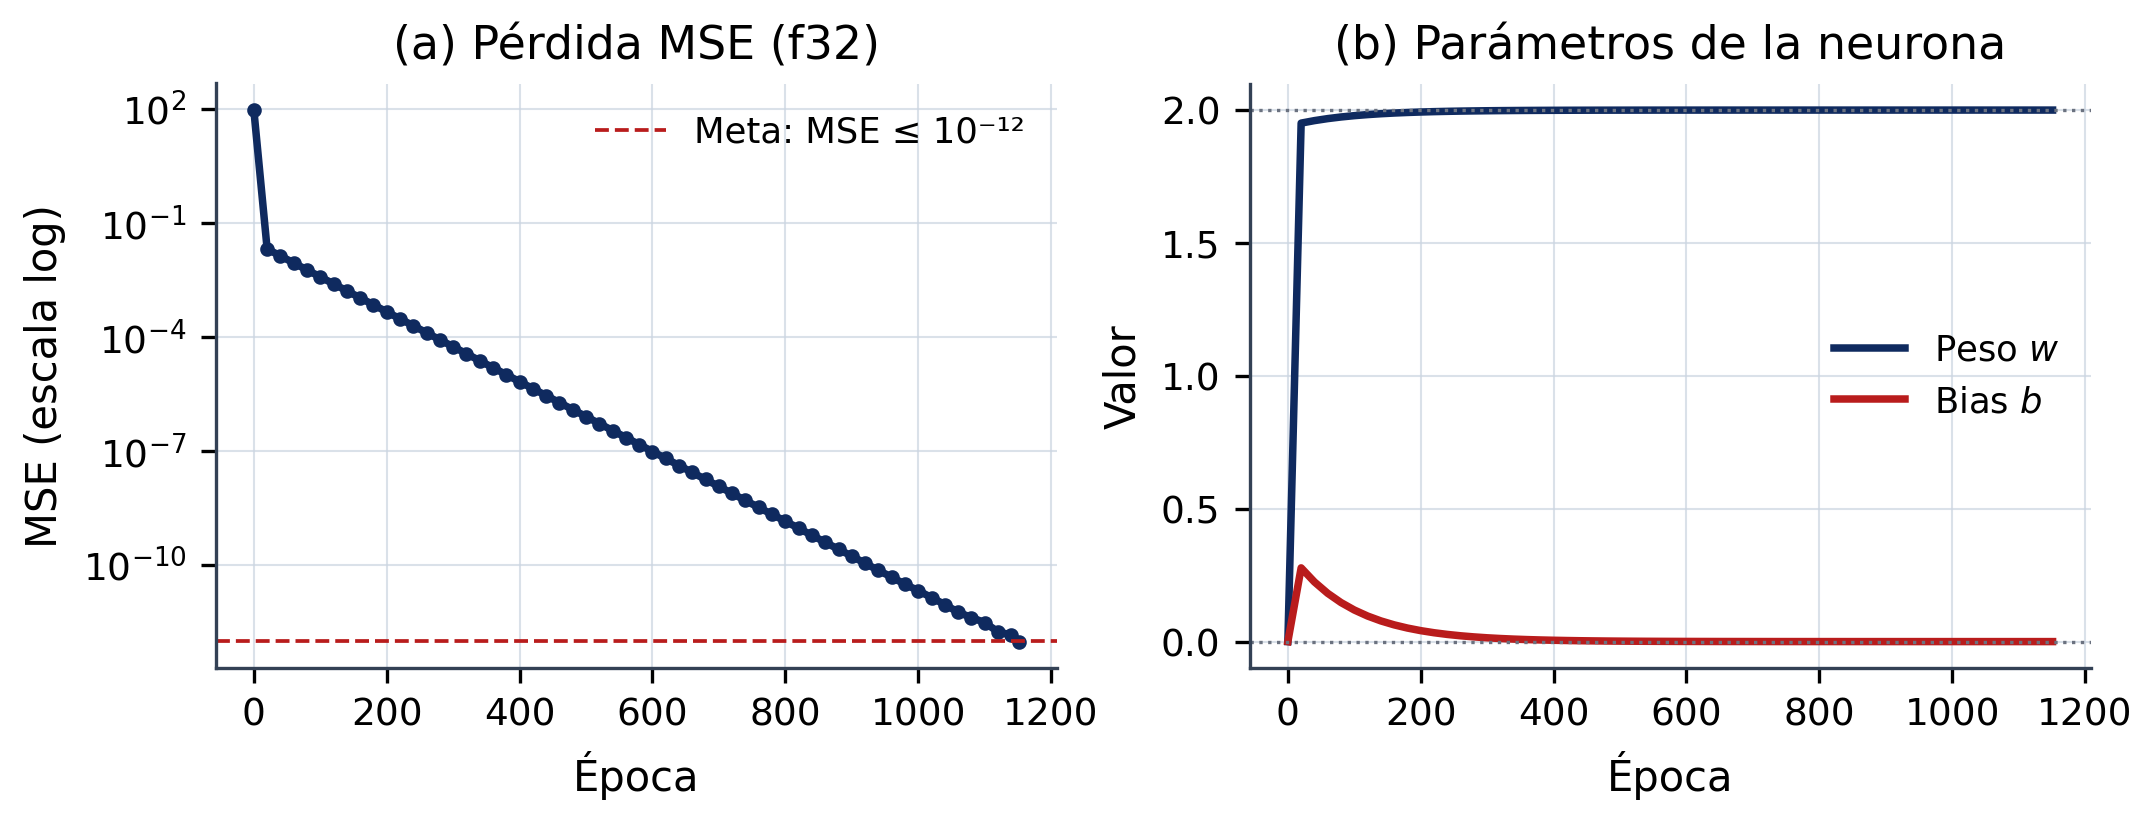
\includegraphics[width=\textwidth]{figuras/fig12_oficial_lineal.png}
\fuente{(a) MSE en escala logarítmica con la meta de $10^{-12}$. (b) Peso y bias. Fuente: \path{resultados/oficial/lineal.csv}.}
\end{figure}

\begin{table}[!htbp]
\caption{Predicciones finales del experimento oficial $y=2x$}\label{tab:of-linpred}
\small
\begin{tabular*}{0.7\textwidth}{@{\extracolsep{\fill}}rrrr@{}}
\toprule
$x$ & Esperado & Predicción & Error \\
\midrule
\TablaOfLinPred
\bottomrule
\end{tabular*}
\fuente{Error $=\hat{y}-y$, con la precisión que imprime el programa. Fuente: \path{resultados/oficial/lineal_predicciones.csv}.}
\end{table}

La pérdida decrece de forma aproximadamente exponencial, como corresponde a un problema cuadrático convexo con una tasa de aprendizaje estable. El salto inicial de 95.33 a 0.02 en las primeras 20 épocas refleja que el peso se acerca a 2 casi de inmediato, mientras el bias, que crece al principio para compensar el error, tarda cientos de épocas en volver a cero. Los errores residuales del orden de $10^{-6}$ de la Tabla~\ref{tab:of-linpred} son el límite práctico de la aritmética \texttt{f32}.

\section{Experimento oficial 2: clasificación booleana}\label{sec:of-bool}
Una neurona Sigmoid aprende a clasificar la entrada 0 como falso y la entrada 1 como verdadero; la clase se decide con el umbral $0.5$. El gradiente de cada muestra es $(p-y)/N$ (Código~\ref{cod:of-bool}), que coincide con la Ecuación~\eqref{eq:ce} para la entropía cruzada binaria. Se entrena durante \OfBoolEpocas{} épocas con $\alpha=\OfBoolAlpha$ y el programa imprime en cada época los gradientes y la actualización de los parámetros.

\lstinputlisting[caption={Gradiente de la clasificación booleana (\texttt{src/experiments/true\_false.rs})},label=cod:of-bool]{generado/codigo/of_bool_muestras.rs}

Al final, $w=\OfBoolW$ y $b=\OfBoolB$; la probabilidad de verdadero es \OfBoolPcero{} para la entrada 0 y \OfBoolPuno{} para la entrada 1, de modo que ambas se clasifican correctamente (exactitud \OfBoolAcc). La Tabla~\ref{tab:of-bool} y la Figura~\ref{fig:of-bool} muestran la evolución.

\begin{table}[!htbp]
\caption{Traza del experimento oficial de clasificación booleana}\label{tab:of-bool}
\footnotesize
\begin{tabular*}{\textwidth}{@{\extracolsep{\fill}}rrrrrrr@{}}
\toprule
Época & $\nabla w$ & $\nabla b$ & $w$ & $b$ & $\sigma(b)$ & $\sigma(w+b)$ \\
\midrule
\TablaOfBool
\bottomrule
\end{tabular*}
\fuente{$\sigma(b)$ y $\sigma(w+b)$ son la probabilidad de verdadero para las entradas 0 y 1, calculadas con los parámetros impresos al final de cada época. Fuente: \path{resultados/oficial/booleano.csv}.}
\end{table}

\begin{figure}[!htbp]
\caption{Parámetros y probabilidades del experimento oficial booleano}\label{fig:of-bool}
\centering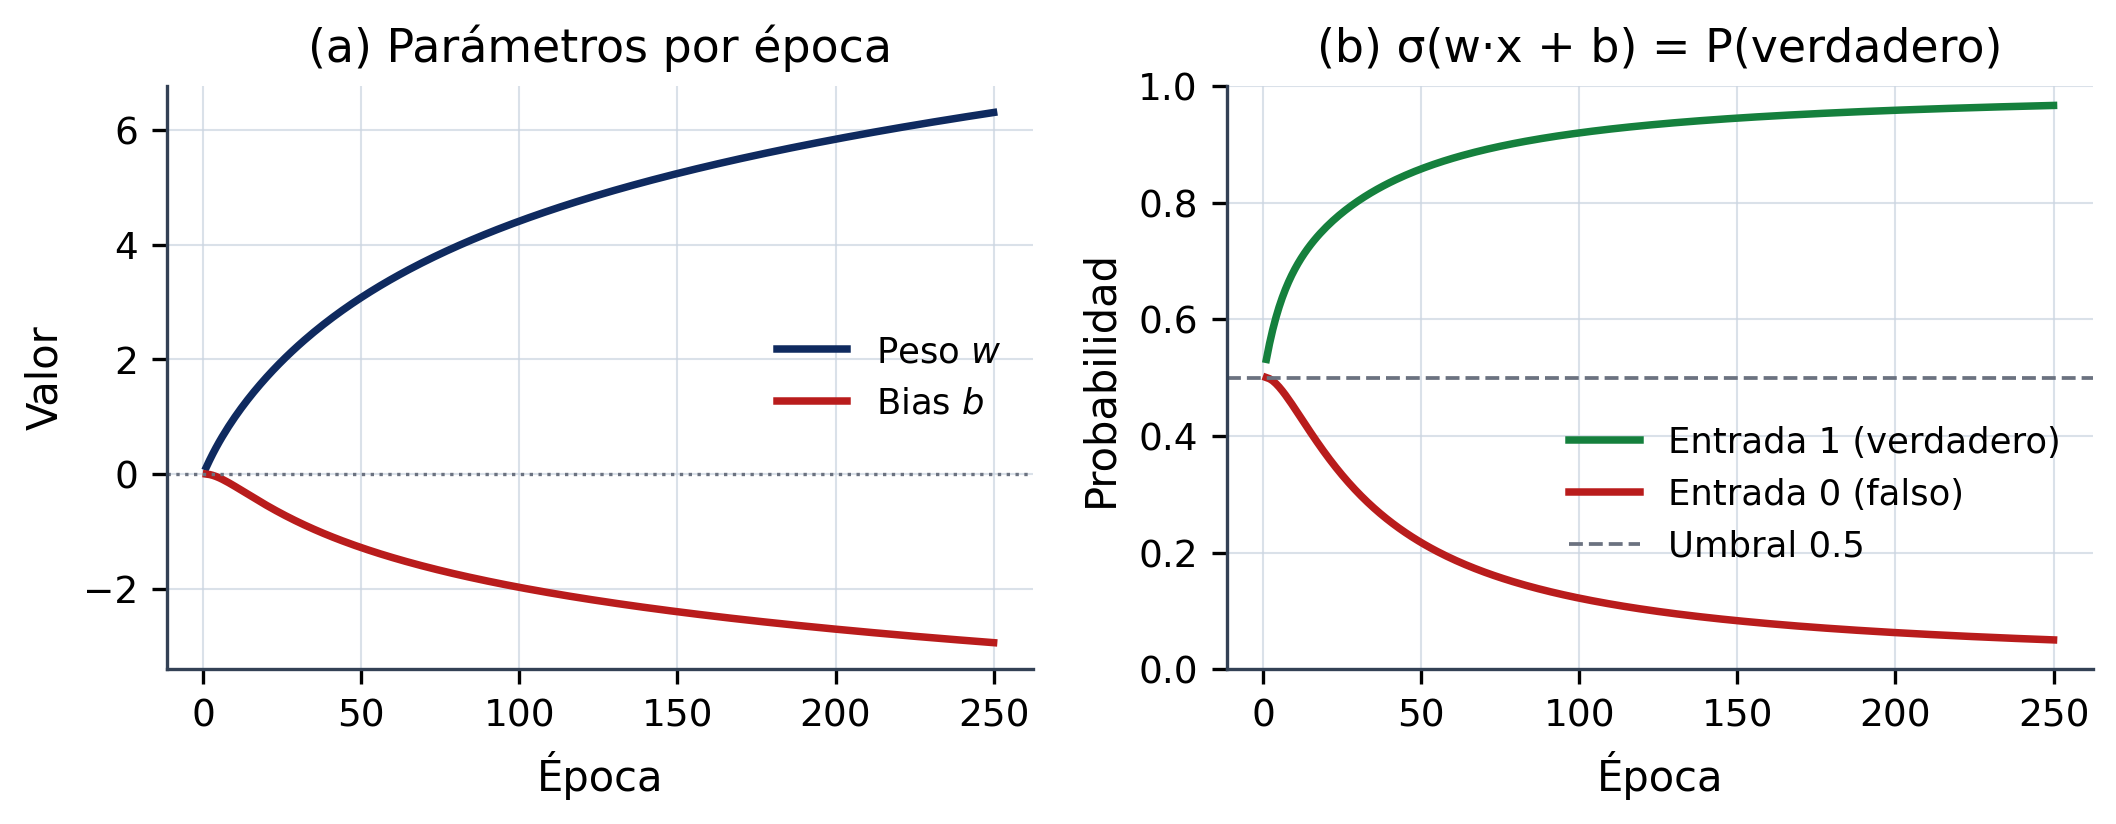
\includegraphics[width=\textwidth]{figuras/fig13_oficial_booleano.png}
\fuente{Fuente: \path{resultados/oficial/booleano.csv}.}
\end{figure}

En la primera época el bias no cambia: con parámetros nulos ambas probabilidades valen $0.5$ y los errores $(0.5-0)$ y $(0.5-1)$ se cancelan. A partir de allí el peso crece y el bias se vuelve negativo, separando las dos probabilidades del umbral. Como el problema es linealmente separable, una sola neurona basta; el problema XOR, que no lo es, se analiza con el motor complementario en la Sección~\ref{sec:exp2}.

\section{Experimento oficial 3: reconocimiento de vocales}\label{sec:of-voc}
Cada vocal se dibuja como una cuadrícula binaria de $5\times5$ (Figura~\ref{fig:of-voc}a) y se aplana en 25 entradas. Una capa de cinco neuronas, una por vocal, produce cinco puntuaciones que softmax convierte en probabilidades; la salida esperada es un vector \emph{one-hot}. El entrenamiento usa \OfVocEpocas{} épocas, $\alpha=\OfVocAlpha$ y descenso de gradiente por lote completo: el Código~\ref{cod:of-voc} acumula los gradientes de las cinco muestras y el Código~\ref{cod:of-vocupd} actualiza las neuronas.

\lstinputlisting[caption={Acumulación de gradientes con softmax (\texttt{src/experiments/vowels.rs})},label=cod:of-voc]{generado/codigo/of_voc_muestras.rs}
\lstinputlisting[caption={Actualización de las cinco neuronas (\texttt{src/experiments/vowels.rs})},label=cod:of-vocupd]{generado/codigo/of_voc_update.rs}

La red reconoce las cinco vocales con una confianza final entre \OfVocConfMin{} y \OfVocConfMax, y la orden \texttt{cargo run -- vocal a} reconoce la A con \OfVocalAProb. La Tabla~\ref{tab:of-voc} y la Figura~\ref{fig:of-voc} muestran la evolución de la probabilidad asignada a la clase correcta.

\begin{table}[!htbp]
\caption{Probabilidad de la clase correcta por época en el experimento oficial de vocales}\label{tab:of-voc}
\footnotesize
\begin{tabular*}{\textwidth}{@{\extracolsep{\fill}}lrrrrrlrr@{}}
\toprule
Vocal & Ép. 1 & Ép. 10 & Ép. 50 & Ép. 100 & Ép. 500 & Reconocida & Confianza (\%) & \texttt{vocal a} (\%) \\
\midrule
\TablaOfVoc
\bottomrule
\end{tabular*}
\fuente{Probabilidades con dos decimales, como las imprime el programa. La última columna es la probabilidad asignada a cada vocal al evaluar el patrón A. Fuente: \path{resultados/oficial/vocales.csv} y \path{resultados/oficial/vocal_a.csv}.}
\end{table}

\begin{figure}[!htbp]
\caption{Patrones, probabilidades y convergencia del experimento oficial de vocales}\label{fig:of-voc}
\centering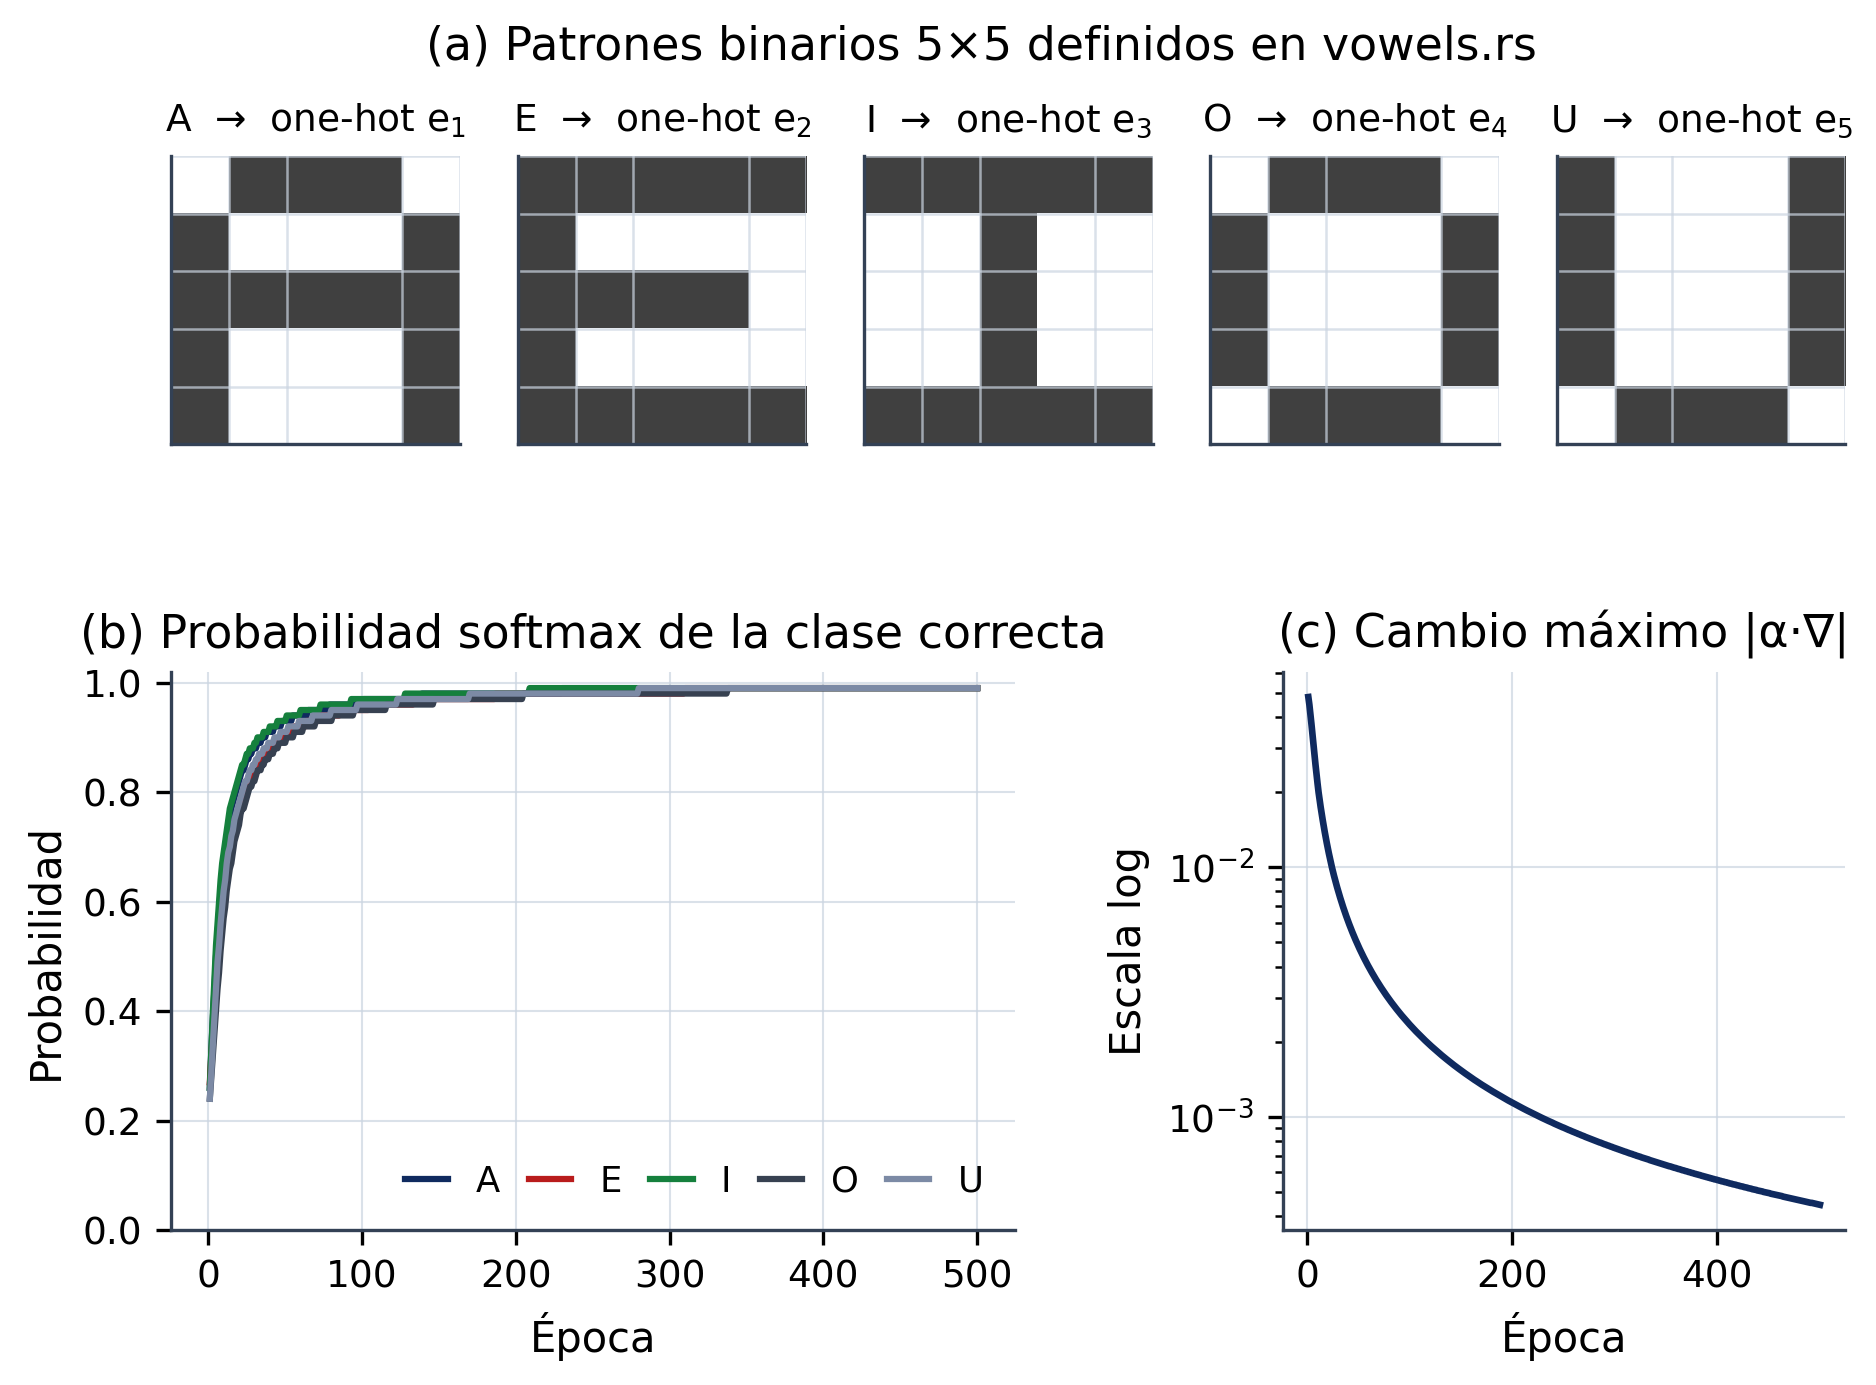
\includegraphics[width=\textwidth]{figuras/fig14_oficial_vocales.png}
\fuente{(c) Mayor cambio absoluto aplicado a un peso o bias en cada época. Fuente: \path{resultados/oficial/vocales.csv}.}
\end{figure}

Desde la primera época la probabilidad más alta corresponde a la vocal correcta, porque cada patrón activa sobre todo los pesos de su propia salida. El resto del entrenamiento aumenta la confianza y el cambio máximo por época desciende hasta \OfVocCambioFin, señal de convergencia. Como el conjunto contiene un único patrón por vocal y se evalúa con los mismos patrones, el resultado demuestra el mecanismo de aprendizaje pero no mide generalización; esa medición se realiza con el motor complementario (Sección~\ref{sec:exp3}).

\section{Tiempos de ejecución del repositorio oficial}\label{sec:of-tiempos}
El programa oficial incluye pausas \texttt{thread::sleep} para que la demostración pueda seguirse en pantalla. Por ello, la Tabla~\ref{tab:of-tiempos} informa dos tiempos: el de pared del binario oficial y el de cómputo de una copia idéntica a la que solo se le quitaron esas pausas (mediana de 5 ejecuciones, incluida la impresión en terminal). El binario \emph{release} ocupa \OfBinKiB~KiB.

\begin{table}[!htbp]
\caption{Tiempos de ejecución del repositorio oficial}\label{tab:of-tiempos}
\small
\begin{tabular*}{\textwidth}{@{\extracolsep{\fill}}llrr@{}}
\toprule
Experimento & Orden & Pared (s) & Cómputo sin pausas (ms) \\
\midrule
\TablaOfTiempos
\bottomrule
\end{tabular*}
\fuente{Linux x86\_64, rustc \OfRustc, perfil \emph{release}. Fuente: \path{resultados/oficial/resumen.csv}.}
\end{table}

\section{Validación complementaria con el motor extendido}\label{sec:complementario}
El repositorio oficial no define pruebas automatizadas ni entrena redes con capas ocultas. El motor extendido, escrito por el equipo en la etapa previa con la misma base matemática, cubre esos aspectos: implementa la retropropagación multicapa (Ecuaciones~\eqref{eq:deltaL}--\eqref{eq:gradW}) en \texttt{f64}, valida los gradientes con 52 pruebas automatizadas, resuelve XOR, evalúa las vocales con ruido y mide tiempos de entrenamiento e inferencia. Sus resultados no sustituyen a los del repositorio oficial: verifican de forma independiente las ecuaciones que este utiliza y muestran hasta dónde puede extenderse.

\subsection{Resultados de verificación}
La suite de pruebas cuenta con 52 pruebas automatizadas (51 en la biblioteca y 1 en la CLI), todas aprobadas. Incluyen valores calculados a mano, errores de dimensión, propiedades matemáticas, determinismo del PRNG, convergencia real de $y=2x$ y XOR, y verificación numérica de gradientes según la Ecuación~\eqref{eq:gradcheck} sobre redes 2-4-1, 3-5-4-2 y 25-10-5. Adicionalmente, \texttt{cargo clippy --all-targets} no reporta advertencias. La salida completa de ambas herramientas se reproduce en el Anexo~\ref{anx:tests}.

\subsection{Prueba de escritorio}\label{sec:escritorio}
La prueba de escritorio registra cada operación de las primeras iteraciones del entrenamiento y permite verificar con calculadora que el código ejecuta exactamente las fórmulas del marco teórico. Para la neurona lineal de $y=2x$ ($\alpha = 0.01$), la primera iteración con $x=1$, $y=2$ y parámetros iniciales $w_0 = \EunoPesoIni$, $b_0 = 0$ es:
\begin{align*}
z &= w_0 x + b_0 = 0.836805\cdot 1 + 0 = 0.836805, & a &= z = 0.836805,\\
e &= a - y = -1.163195, & \mathcal{L} &= e^2 = 1.353022,\\
\delta &= 2e\cdot f'(z) = -2.326389, & \partial\mathcal{L}/\partial w &= \delta\, x = -2.326389,\\
w_1 &= w_0 - \alpha\,\delta x = 0.860069, & b_1 &= b_0 - \alpha\,\delta = 0.023264.
\end{align*}
La Tabla~\ref{tab:escritorio} resume las diez primeras iteraciones (dos épocas) y la Figura~\ref{fig:escritorio} muestra la evolución de los parámetros a lo largo de esas iteraciones.

\begin{table}[!htbp]
\caption{Prueba de escritorio de la neurona lineal para $y=2x$ (primeras 10 iteraciones)}\label{tab:escritorio}
\footnotesize\setlength{\tabcolsep}{3.5pt}
\begin{tabular*}{\textwidth}{@{\extracolsep{\fill}}rrrrrrrrrr@{}}
\toprule
It. & $x$ & $y$ & $w$ & $b$ & $z$ & $e$ & $\partial\mathcal{L}/\partial w$ & $w'$ & $b'$ \\
\midrule
\TablaEscritorio
\bottomrule
\end{tabular*}
\fuente{$e = \hat{y}-y$; $w'$ y $b'$ son los parámetros después de la actualización. Fuente: \path{resultados/prueba_escritorio.csv}.}
\end{table}

\begin{figure}[!htbp]
\caption{Evolución de los parámetros durante la prueba de escritorio}\label{fig:escritorio}
\centering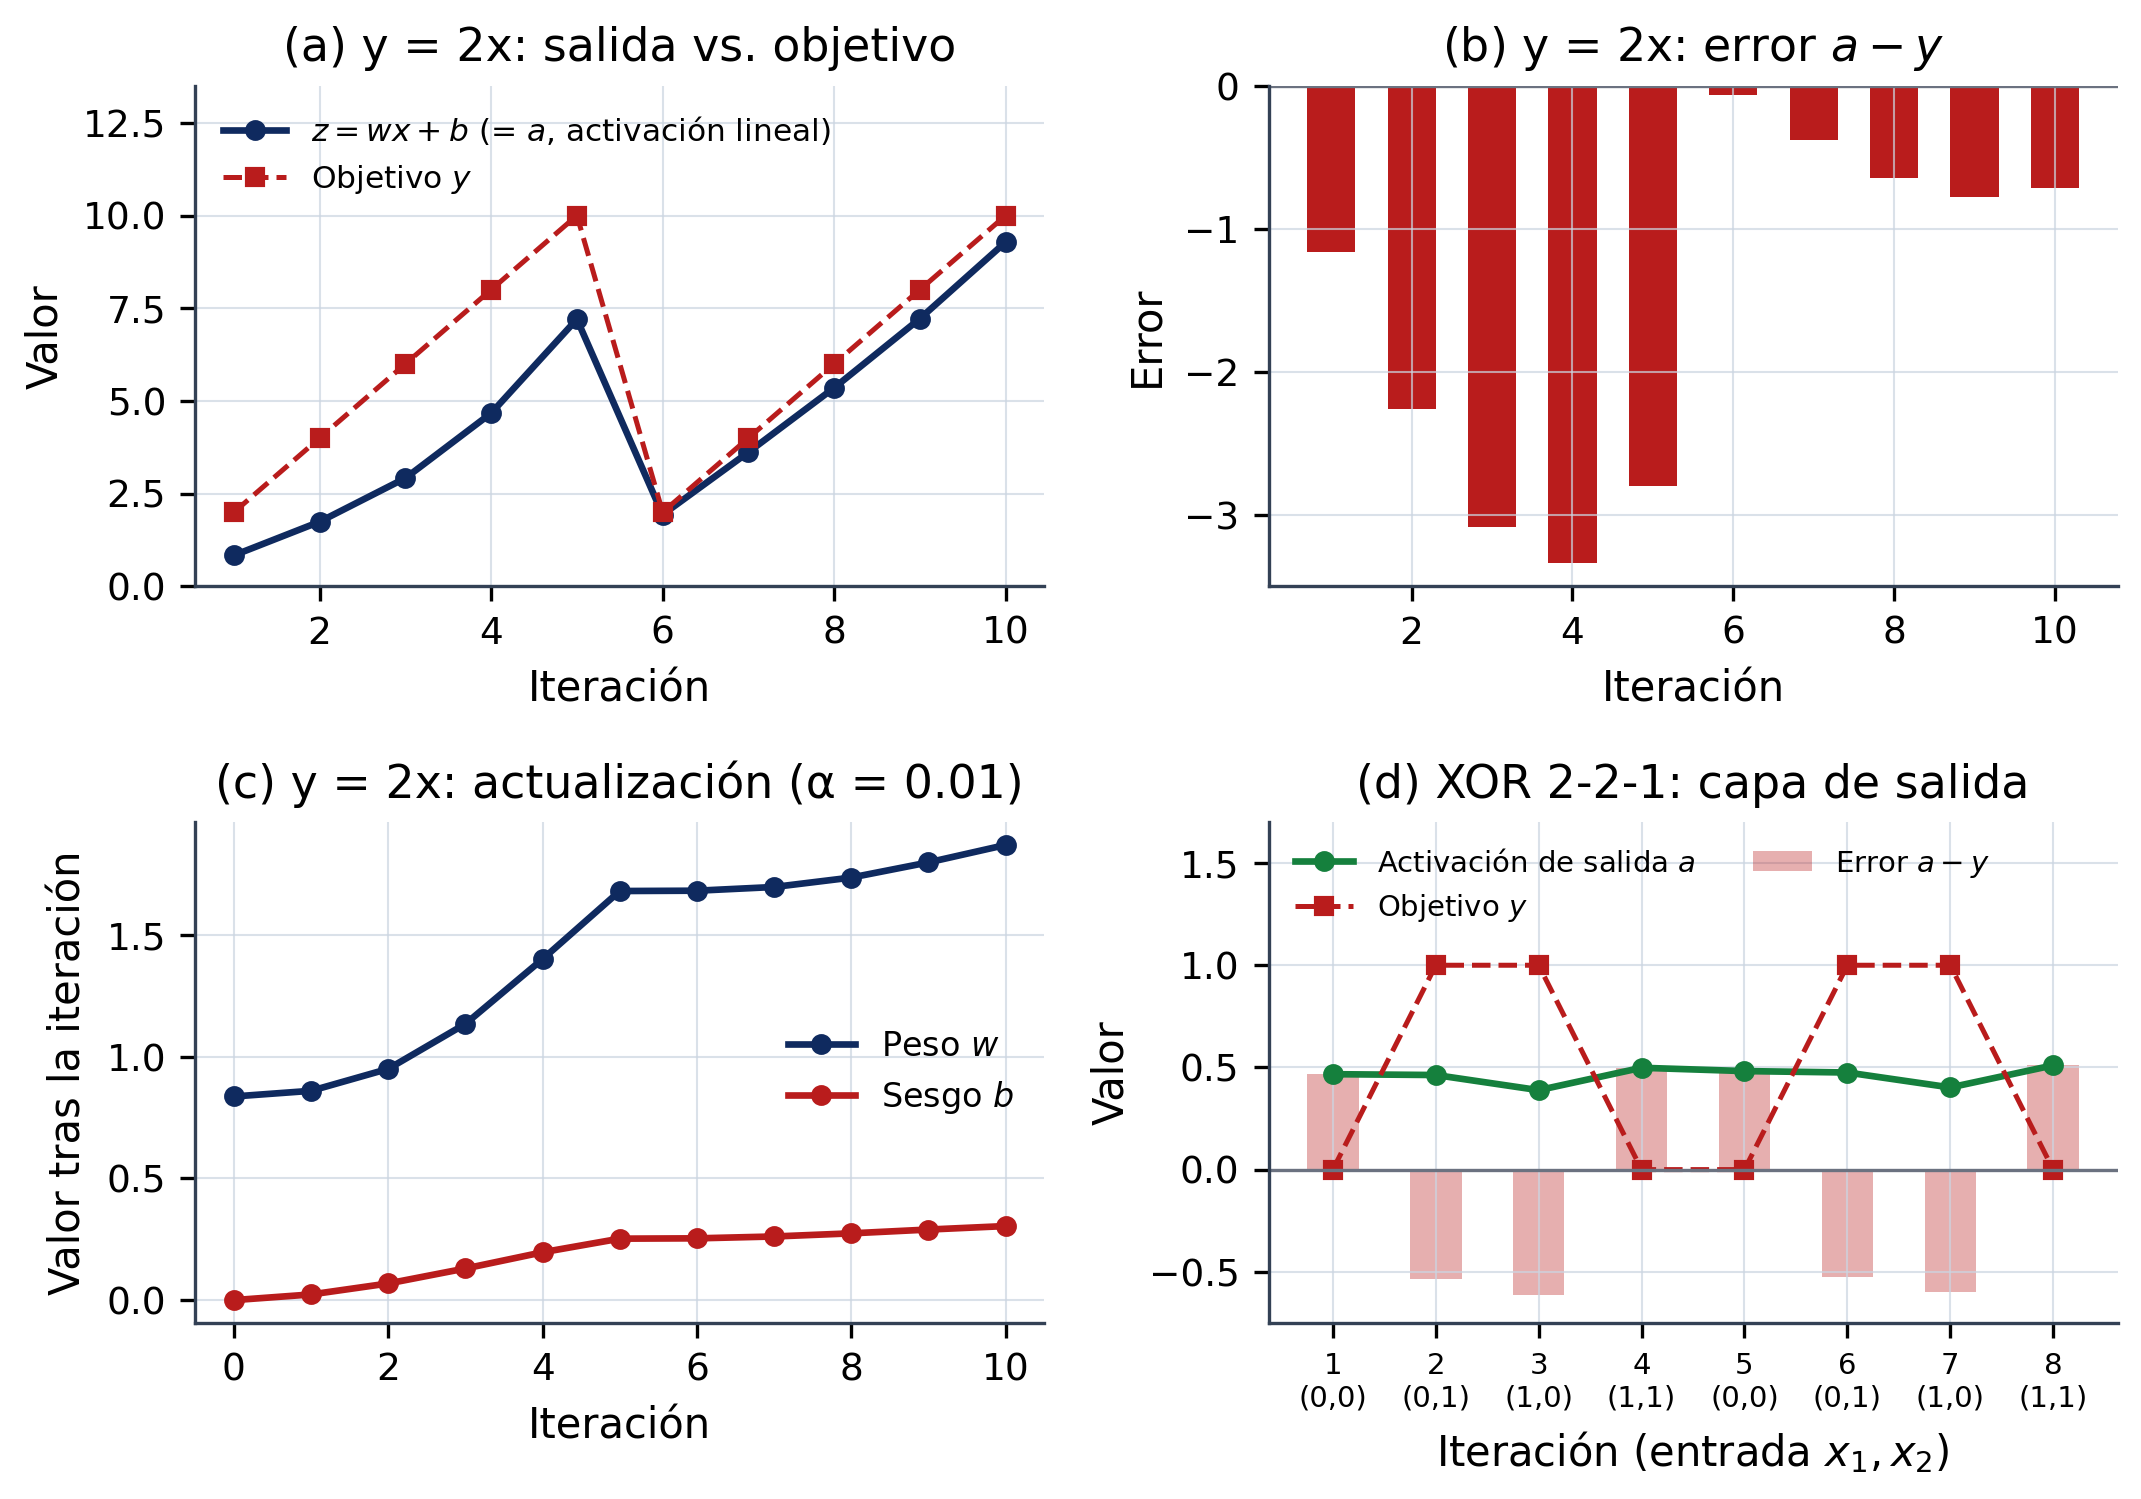
\includegraphics[width=\textwidth]{figuras/fig11_prueba_escritorio.png}
\fuente{Valores de la traza registrada por el binario en \path{resultados/prueba_escritorio.csv}.}
\end{figure}

La traza también incluye las primeras iteraciones de una red \PeXorEsc{} y contiene \PeFilas{} filas en total. La Tabla~\ref{tab:escritorio-xor} muestra las dos primeras iteraciones de esa red. En la primera iteración, la entrada $(0,0)$ anula las sumas ponderadas de la capa oculta, cuyas neuronas producen exactamente $\sigma(0)=0.5$; por ello sus gradientes de pesos son nulos y solo se actualizan los sesgos, comportamiento que coincide con la Ecuación~\eqref{eq:gradW}, pues $\partial\mathcal{L}/\partial w_{ji} = \delta_j\,x_i = 0$ cuando $x_i=0$.

\begin{table}[!htbp]
\caption{Prueba de escritorio de la red XOR 2-2-1 (dos primeras iteraciones)}\label{tab:escritorio-xor}
\footnotesize\setlength{\tabcolsep}{3.5pt}
\begin{tabular*}{\textwidth}{@{\extracolsep{\fill}}rlrrrrrrrr@{}}
\toprule
It. & Entrada & $y$ & Capa & Neurona & $z$ & $a$ & $\delta$ & $b$ & $b'$ \\
\midrule
\TablaEscritorioXor
\bottomrule
\end{tabular*}
\fuente{Capa 1: oculta; capa 2: salida. $\alpha = 0.5$. Fuente: \path{resultados/prueba_escritorio.csv}.}
\end{table}

\subsection{Regresión $y=2x$ en doble precisión}\label{sec:exp1}
El motor complementario repite la regresión con 5 pares $(x,2x)$, peso inicial aleatorio $w_0=\EunoPesoIni$, $\alpha=\EunoAlpha$ y \EunoEpocas{} épocas de descenso de gradiente por muestra. Termina con $w=\EunoPesoFin$ y un MSE de \EunoMseFin, frente a \OfLinMseFin{} del repositorio oficial. La diferencia de cinco órdenes de magnitud se debe al tipo numérico: con \texttt{f64} el error puede descender hasta cerca de $10^{-18}$, mientras que \texttt{f32} representa unas siete cifras decimales y el repositorio oficial se detiene, además, al alcanzar su meta de $10^{-12}$. Ambas implementaciones llegan a la solución analítica $w=2$, $b=0$.

\subsection{Compuerta XOR: necesidad de una capa oculta}\label{sec:exp2}
El repositorio oficial no incluye XOR; el motor complementario lo aborda porque reproduce el problema que detuvo la investigación en redes neuronales durante la década de 1970. La función XOR devuelve 1 cuando sus dos entradas binarias son distintas. Se comparan un perceptrón de una capa (2-1, Sigmoid) y una red multicapa 2-4-1 (Sigmoid/Sigmoid), ambos entrenados durante \EdosEpocas{} épocas con $\alpha=\EdosAlpha$. Además, la red 2-4-1 se entrena con tres tasas de aprendizaje: baja ($0.01$), óptima ($0.5$) y alta ($50$).

\subsubsection*{Perceptrón frente a red multicapa}
El perceptrón terminó con MSE de \EdosMsePer{} y exactitud de \EdosAccPer, mientras que la red multicapa alcanzó MSE de \EdosMseMul{} y exactitud de \EdosAccMul{}. La Tabla~\ref{tab:exp2} presenta las predicciones finales y la Figura~\ref{fig:exp2conv} compara las curvas de pérdida.

\begin{table}[!htbp]
\caption{Predicciones finales para XOR}\label{tab:exp2}
\small
\begin{tabular*}{\textwidth}{@{\extracolsep{\fill}}lrrr@{}}
\toprule
Entrada & Objetivo & Perceptrón 2-1 & Multicapa 2-4-1 \\
\midrule
\TablaEdos
\bottomrule
\end{tabular*}
\fuente{Se clasifica como 1 cuando la salida es $\ge 0.5$. Fuente: \path{resultados/exp2_xor.csv}.}
\end{table}

\begin{figure}[!htbp]
\caption{Curvas de pérdida del perceptrón 2-1 y de la red multicapa 2-4-1 en XOR}\label{fig:exp2conv}
\centering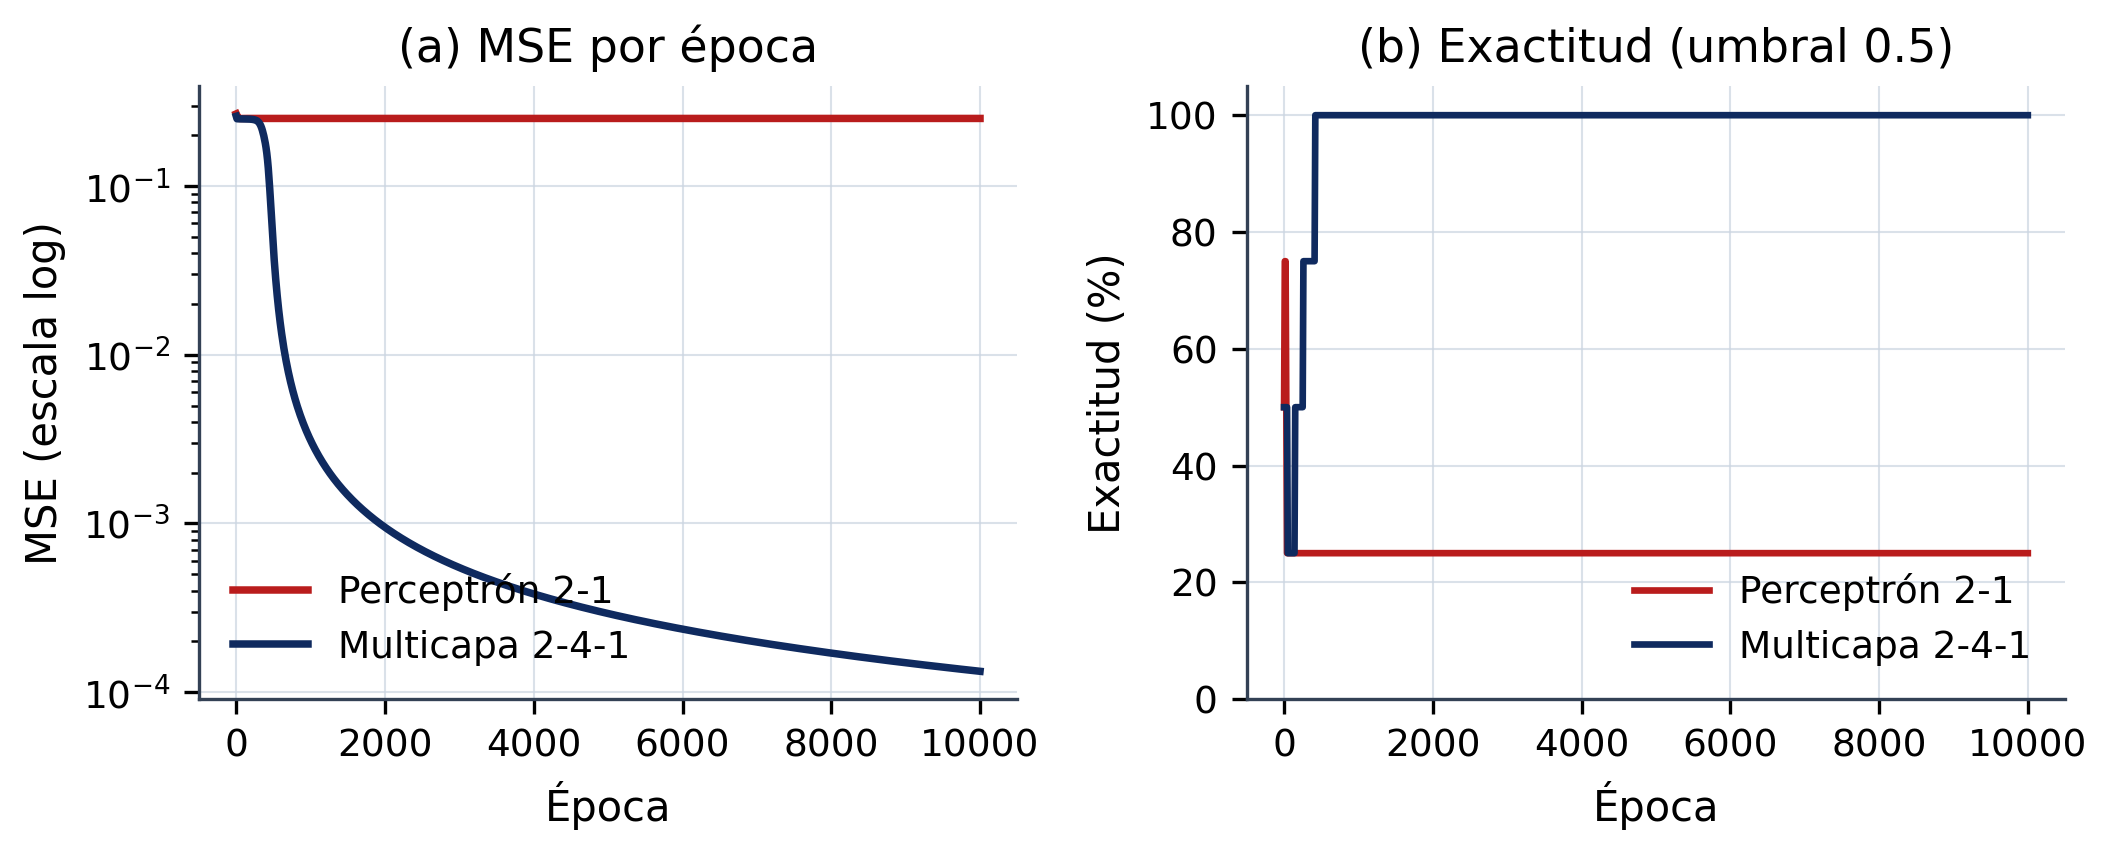
\includegraphics[width=\textwidth]{figuras/fig04_exp2_xor_convergencia.png}
\fuente{Eje vertical en escala logarítmica. Fuente: \path{resultados/exp2_xor.csv}.}
\end{figure}

La Figura~\ref{fig:frontera} muestra la salida de ambos modelos sobre una malla del plano de entradas. El perceptrón solo puede trazar una frontera recta, que deja necesariamente a un punto de cada clase del lado equivocado; la red multicapa, en cambio, construye una región de decisión no lineal que separa correctamente las cuatro entradas.

\begin{figure}[!htbp]
\caption{Fronteras de decisión aprendidas para XOR}\label{fig:frontera}
\centering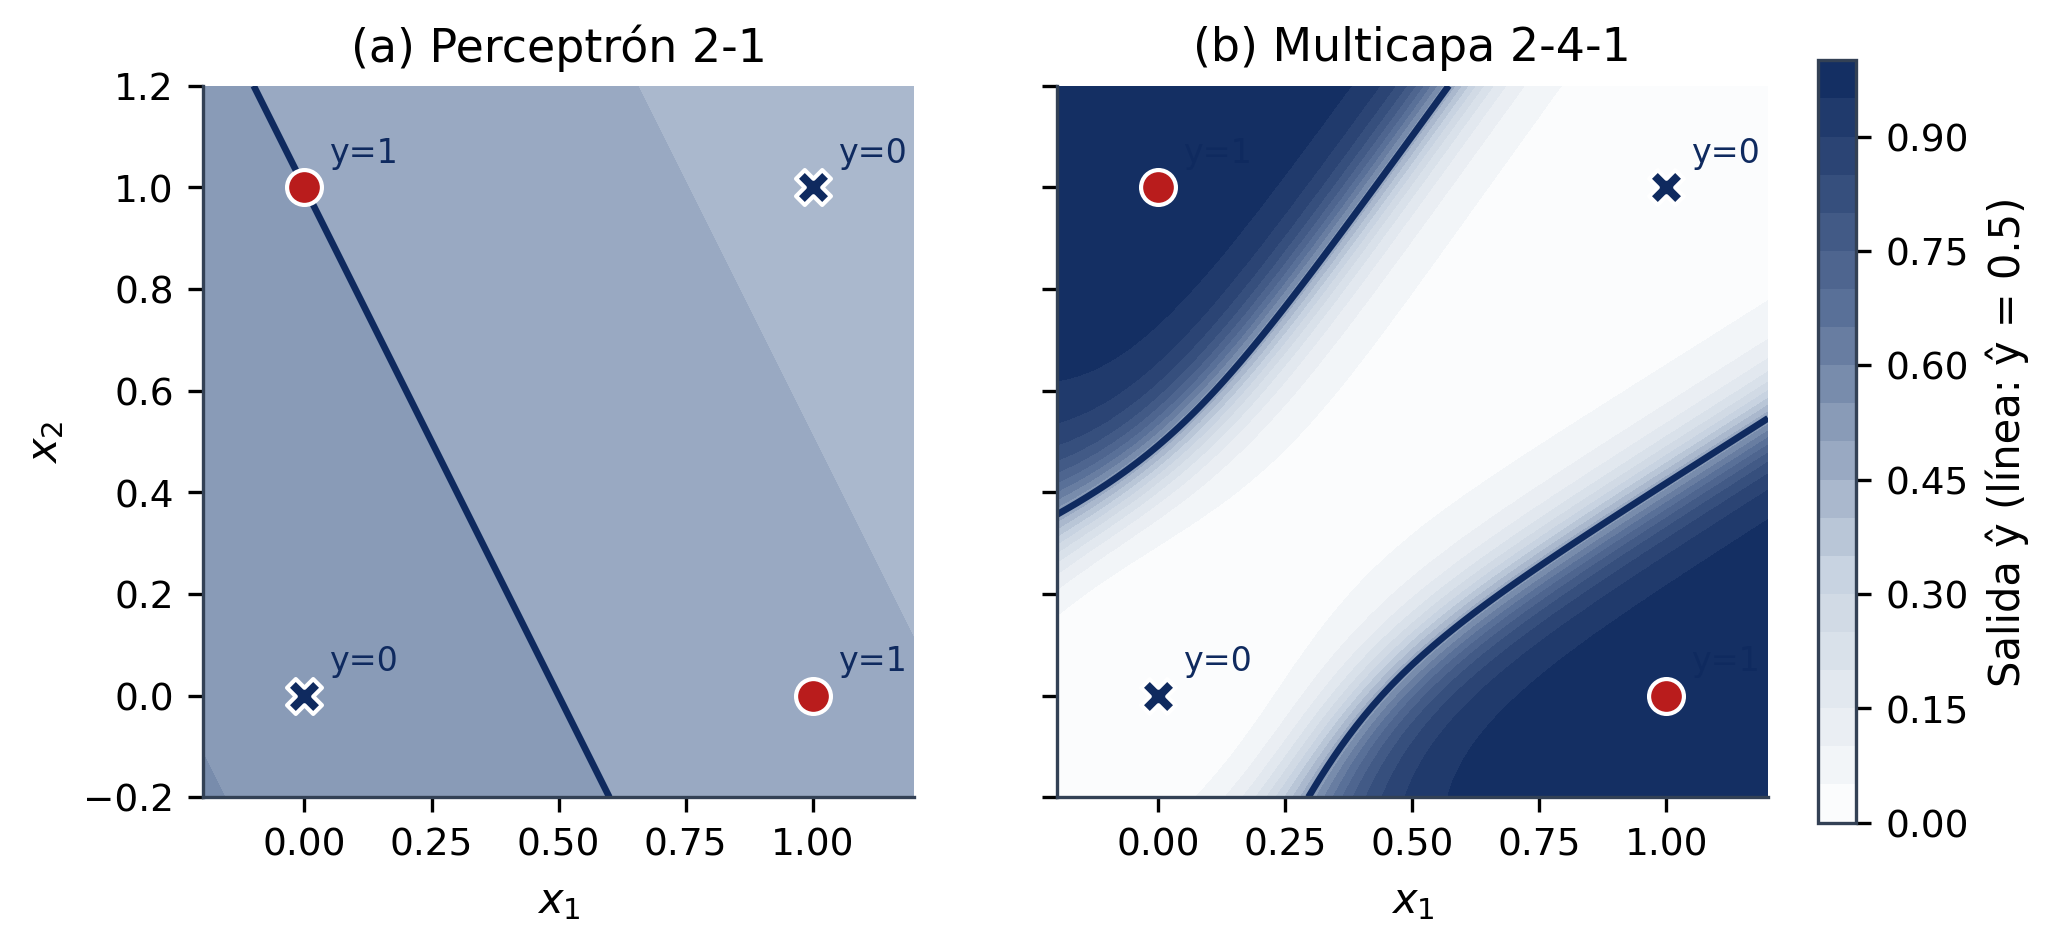
\includegraphics[width=\textwidth]{figuras/fig06_exp2_xor_frontera.png}
\fuente{(a) Perceptrón 2-1. (b) Red multicapa 2-4-1. La línea indica $\hat{y}=0.5$. Fuente: \path{resultados/exp2_xor_frontera.csv}.}
\end{figure}

\subsubsection*{Efecto de la tasa de aprendizaje}
La Tabla~\ref{tab:exp2lr} y la Figura~\ref{fig:lr} resumen el comportamiento de la red 2-4-1 con las tres tasas de aprendizaje estudiadas.

\begin{table}[!htbp]
\caption{Efecto de la tasa de aprendizaje en la red 2-4-1 para XOR}\label{tab:exp2lr}
\small
\begin{tabular*}{\textwidth}{@{\extracolsep{\fill}}lrrrl@{}}
\toprule
Escenario & $\alpha$ & MSE final & Exactitud & Época de convergencia \\
\midrule
\TablaEdosLr
\bottomrule
\end{tabular*}
\fuente{Convergencia: primera época con MSE $<0.01$. Fuente: \path{resultados/exp2_xor_lr.csv}.}
\end{table}

\begin{figure}[!htbp]
\caption{Curvas de pérdida de la red 2-4-1 con tasas de aprendizaje baja, óptima y alta}\label{fig:lr}
\centering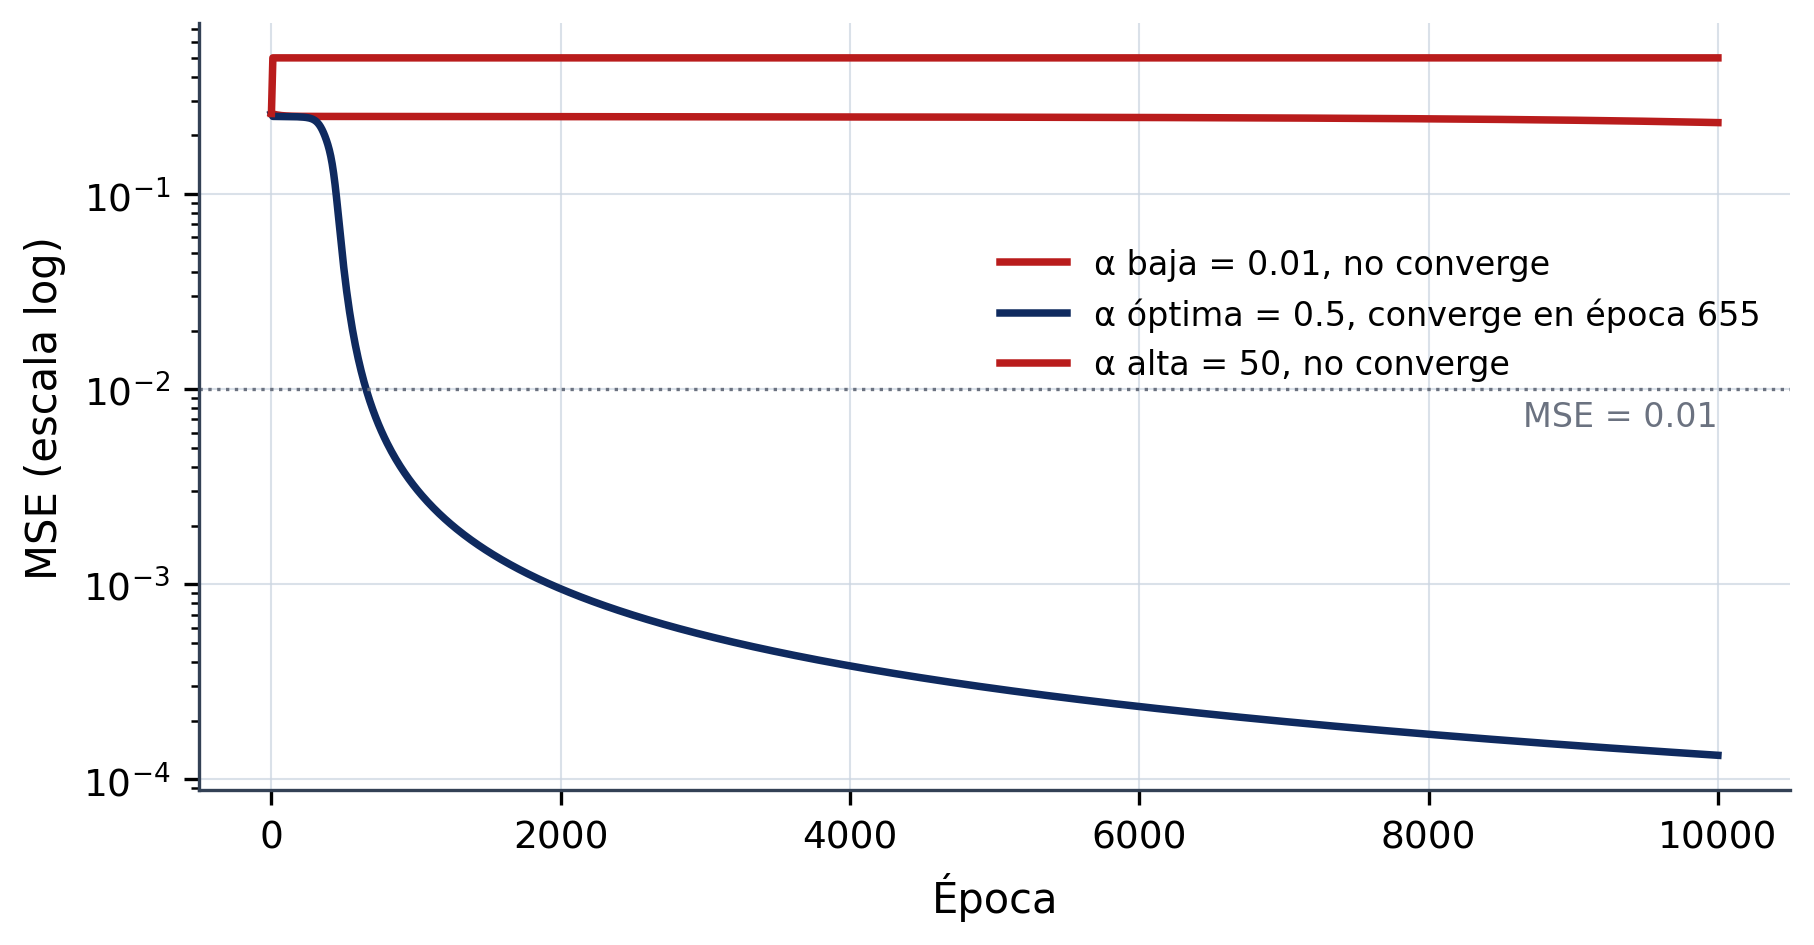
\includegraphics[width=\textwidth]{figuras/fig05_exp2_xor_learning_rates.png}
\fuente{Fuente: \path{resultados/exp2_xor_lr.csv}.}
\end{figure}

\subsubsection*{Análisis}
El perceptrón no puede resolver XOR porque sus cuatro puntos no son linealmente separables, como se demostró en el Capítulo~\ref{cap:marco}. Su MSE se estanca cerca de $0.25$, valor que corresponde a predecir aproximadamente $0.5$ para todas las entradas: el optimizador encuentra el compromiso menos malo entre clases que no puede separar. La capa oculta de la red 2-4-1 transforma el espacio de entrada en una representación en la que las clases sí son separables, lo que confirma empíricamente el teorema de aproximación universal \citep{cybenko1989}.

Respecto a la tasa de aprendizaje, con $\alpha=0.01$ la red apenas avanza en \EdosEpocas{} épocas (MSE de \EdosMseBaja); con $\alpha=0.5$ converge en la época \EdosConvOptima; y con $\alpha=50$ los pasos son tan grandes que las neuronas Sigmoid se saturan, sus derivadas se anulan y el aprendizaje se detiene con MSE de \EdosMseAlta. Este último valor equivale a que la red produzca salidas saturadas en 0 o en 1 que aciertan exactamente la mitad de los casos. El resultado ilustra que la tasa de aprendizaje no es un detalle de configuración, sino un hiperparámetro que determina si el entrenamiento converge \citep{ruder2016}.

\subsection{Vocales con ruido y conjunto de prueba separado}\label{sec:exp3}
El experimento oficial de vocales evalúa los mismos cinco patrones con los que entrena. El motor complementario extiende el problema con una red 25-10-5, variantes ruidosas y un conjunto de prueba separado, lo que permite medir generalización.

\subsubsection*{Conjunto de datos}
Cada vocal se representa como una matriz binaria de $5\times5$ (Figura~\ref{fig:dataset}), aplanada en un vector de 25 entradas. La salida usa codificación \emph{one-hot} de 5 posiciones. El conjunto de entrenamiento contiene \EtresNEnt{} muestras (los 5 prototipos y 4 variantes por vocal con un píxel invertido). El conjunto de prueba contiene \EtresNPru{} muestras distintas de las de entrenamiento: 10 variantes por vocal para cada nivel de ruido de 1 a 5 píxeles invertidos. El ruido se genera invirtiendo $k$ píxeles elegidos mediante el barajado de Fisher--Yates (Código~\ref{cod:ruido}).

\begin{figure}[!htbp]
\caption{Prototipos binarios $5\times5$ y ejemplos con ruido del conjunto de vocales}\label{fig:dataset}
\centering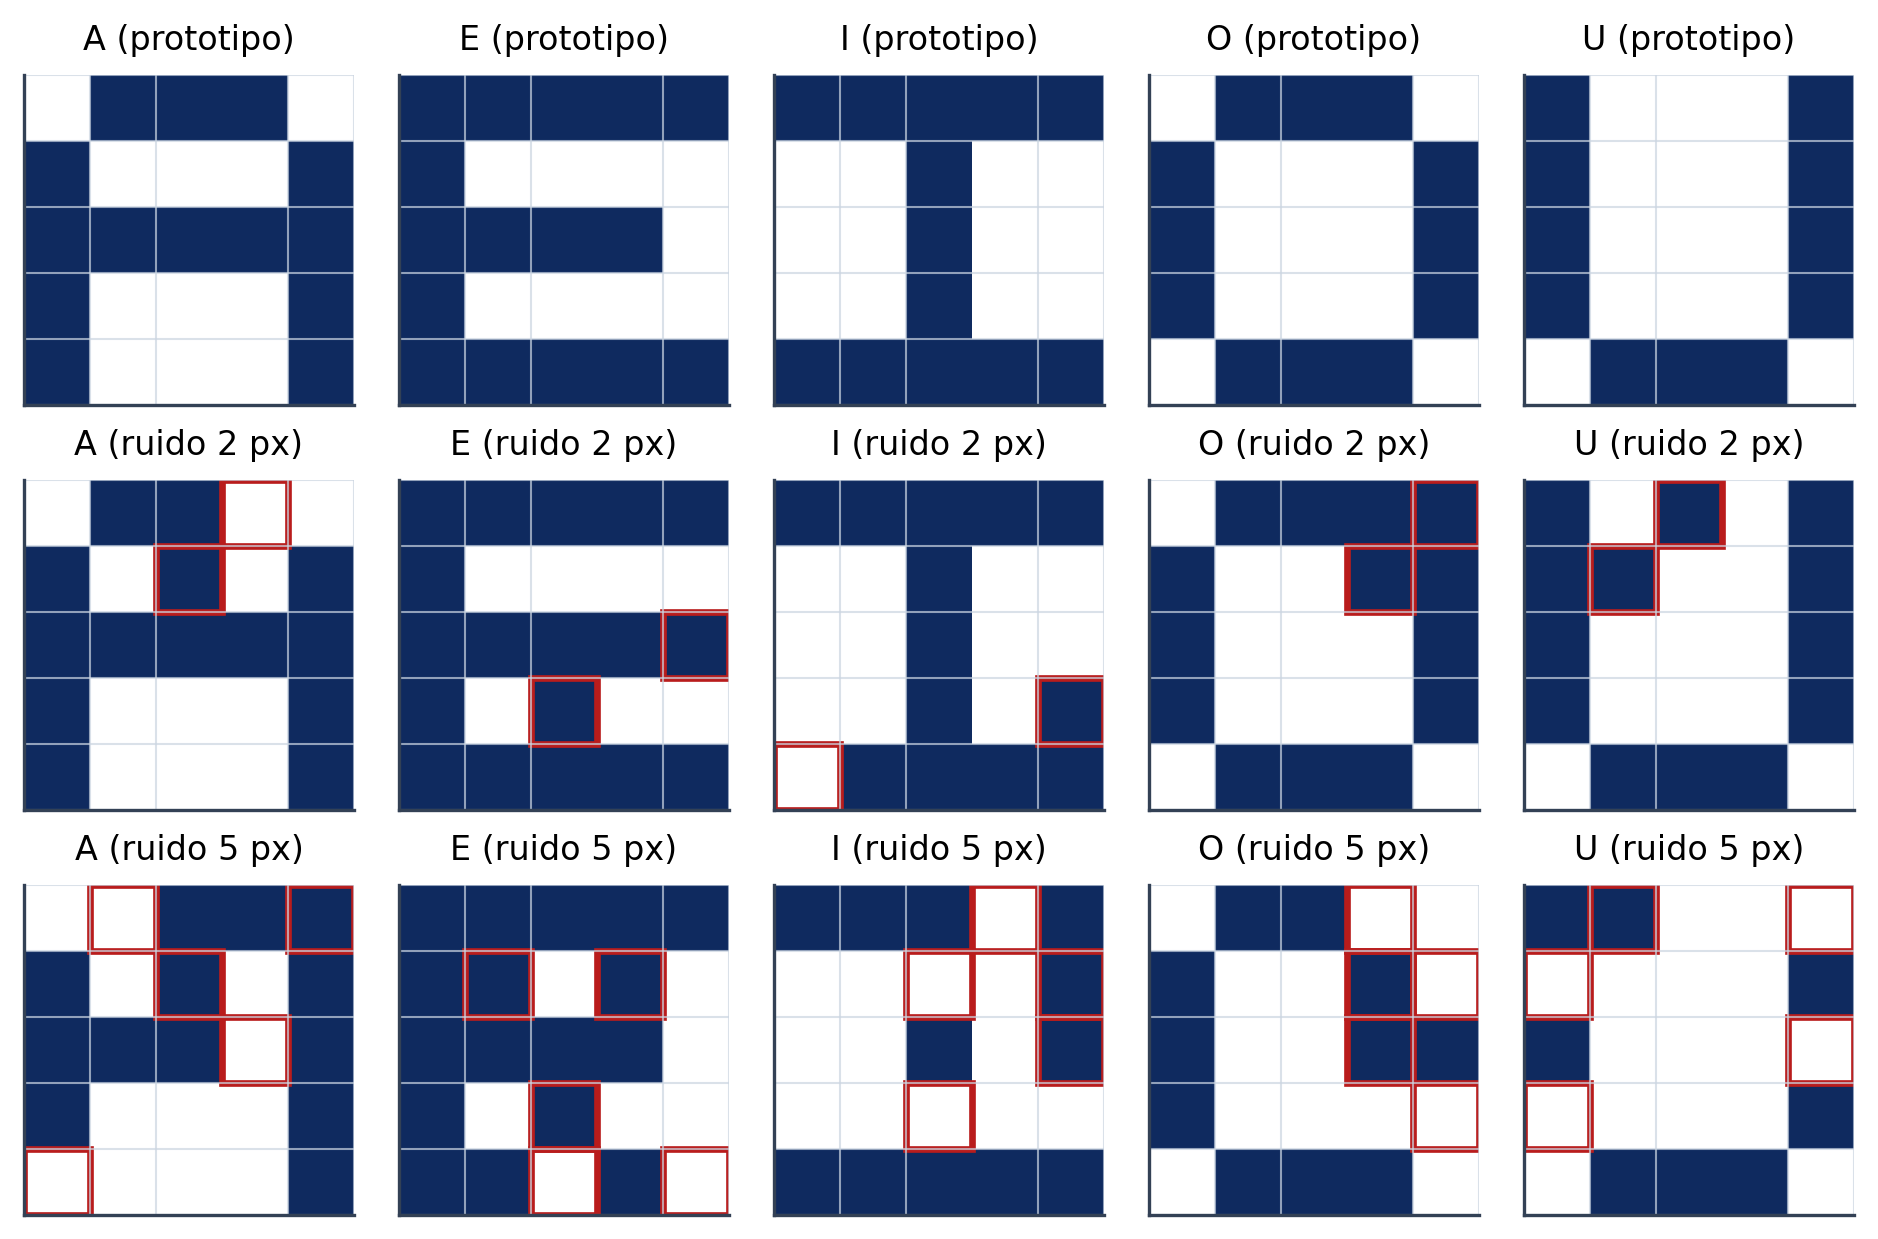
\includegraphics[width=\textwidth,height=0.42\textheight,keepaspectratio]{figuras/fig07_exp3_dataset_vocales.png}
\fuente{Celda oscura = 1, celda clara = 0. Fuente: \path{resultados/dataset_vocales.csv}.}
\end{figure}

\lstinputlisting[caption={Variantes con $k$ píxeles invertidos (\texttt{src/experiments/exp3\_vocales.rs})},label=cod:ruido]{generado/codigo/con_ruido.rs}

\subsubsection*{Resultados}
La red 25-10-5 (Sigmoid/Sigmoid, 315 parámetros) se entrenó durante \EtresEpocas{} épocas con $\alpha=\EtresAlpha$. Alcanzó en entrenamiento un MSE de \EtresMseEnt{} con exactitud de \EtresAccEnt, y en prueba un MSE de \EtresMsePru{} con exactitud de \EtresAccPru. La Figura~\ref{fig:exp3train} muestra la evolución del error, la Tabla~\ref{tab:ruido} desglosa la exactitud por nivel de ruido, y la Tabla~\ref{tab:confusion} y la Figura~\ref{fig:confusion} presentan la matriz de confusión.

\begin{figure}[!htbp]
\caption{Evolución del error de entrenamiento y de prueba en la clasificación de vocales}\label{fig:exp3train}
\centering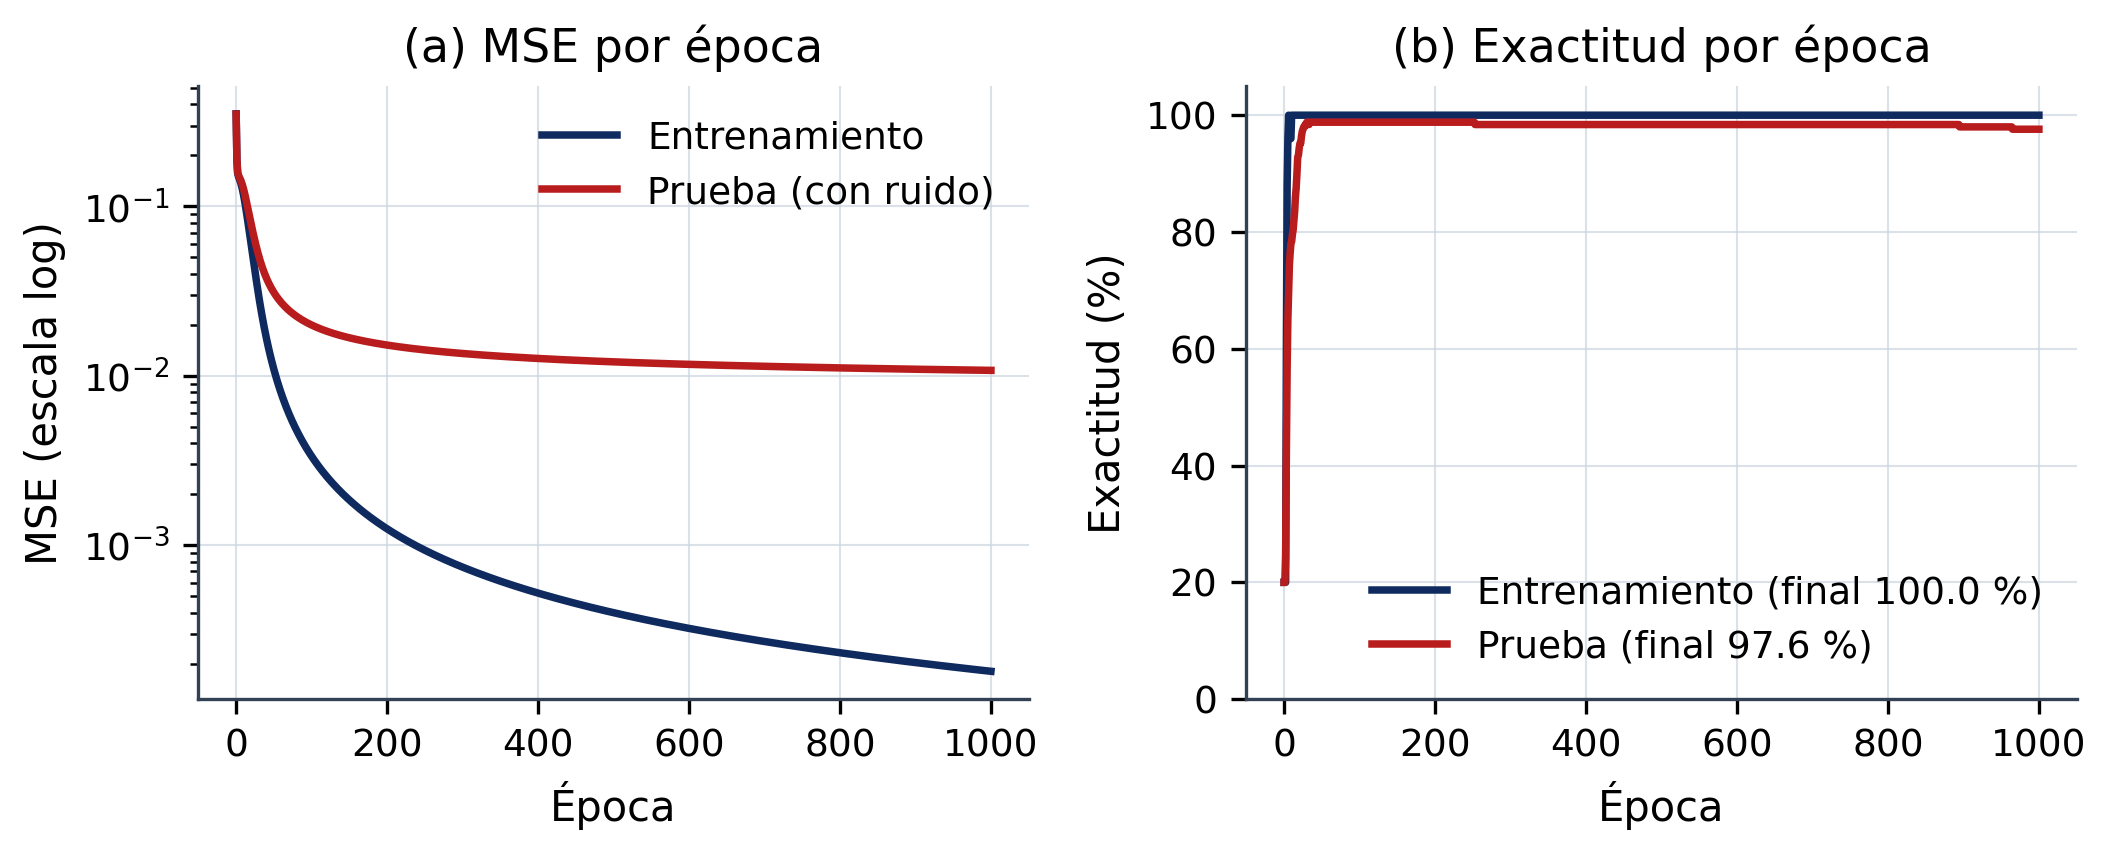
\includegraphics[width=\textwidth]{figuras/fig08_exp3_vocales_entrenamiento.png}
\fuente{Fuente: \path{resultados/exp3_vocales.csv}.}
\end{figure}

\begin{table}[!htbp]
\caption{Exactitud de prueba por nivel de ruido}\label{tab:ruido}
\small
\begin{tabular*}{0.7\textwidth}{@{\extracolsep{\fill}}rrr@{}}
\toprule
Píxeles invertidos & Muestras & Exactitud \\
\midrule
\TablaEtresRuido
\bottomrule
\end{tabular*}
\fuente{Fuente: \path{resultados/resumen.csv}.}
\end{table}

\begin{table}[!htbp]
\caption{Matriz de confusión del conjunto de prueba}\label{tab:confusion}
\small
\begin{tabular*}{0.7\textwidth}{@{\extracolsep{\fill}}l ccccc@{}}
\toprule
Real / Predicha & A & E & I & O & U \\
\midrule
\TablaConfusion
\bottomrule
\end{tabular*}
\fuente{Filas: clase real; columnas: clase predicha. Fuente: \path{resultados/exp3_confusion.csv}.}
\end{table}

\begin{figure}[!htbp]
\caption{Matriz de confusión del Experimento 3}\label{fig:confusion}
\centering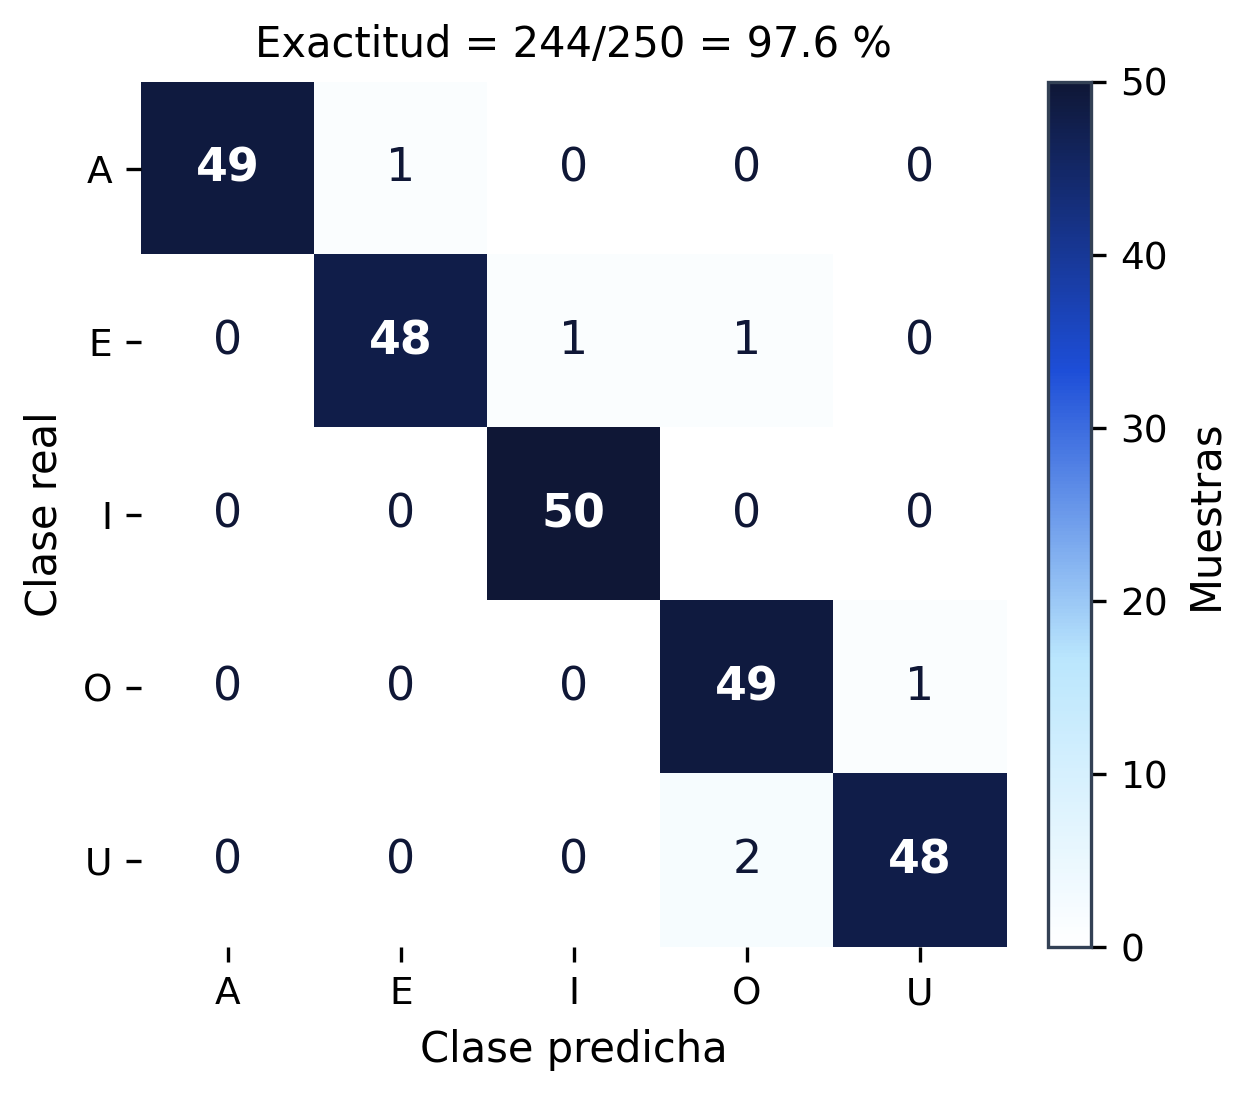
\includegraphics[width=0.72\textwidth]{figuras/fig09_exp3_matriz_confusion.png}
\fuente{La diagonal concentra las clasificaciones correctas. Fuente: \path{resultados/exp3_confusion.csv}.}
\end{figure}

\subsubsection*{Análisis}
La red clasifica sin errores todas las muestras con hasta 3 píxeles invertidos (12\,\% de la imagen), aunque durante el entrenamiento solo vio variantes con un píxel alterado. Con 4 y 5 píxeles invertidos (16\,\% y 20\,\%) la exactitud desciende al 94\,\%. Los errores se concentran entre pares de vocales visualmente parecidas: O y U comparten los laterales y la base, y E comparte la columna izquierda con otras letras. La subsección siguiente examina cada uno de esos errores. La diferencia entre el MSE de entrenamiento y el de prueba es la esperada al evaluar con niveles de ruido mayores que los de entrenamiento, y no impide una exactitud global de \EtresAccPru. El comportamiento es coherente con la representación aprendida y muestra la capacidad de generalización del modelo frente a perturbaciones no observadas.

\subsubsection*{Análisis de los errores de clasificación}
La matriz de confusión registra 6 errores sobre 250 muestras, todos con 4 o 5 píxeles invertidos: 1 A clasificada como E, 1 E como I, 1 E como O, 1 O como U y 2 U como O. Para explicarlos se calculó la distancia de Hamming entre los prototipos, es decir, el número de píxeles en que difieren dos vocales (Tabla~\ref{tab:hamming}). Cuando una muestra tiene $k$ píxeles invertidos, su distancia al prototipo correcto es $k$, y puede quedar tan cerca de otra vocal como de la propia si los píxeles invertidos coinciden con las posiciones en que ambas difieren.

\begin{table}[!htbp]
\caption{Distancia de Hamming entre los prototipos $5\times5$ de las vocales}\label{tab:hamming}
\small
\begin{tabular*}{0.6\textwidth}{@{\extracolsep{\fill}}l ccccc@{}}
\toprule
Vocal & A & E & I & O & U \\
\midrule
\TablaHamming
\bottomrule
\end{tabular*}
\fuente{Número de píxeles distintos entre prototipos. Calculado desde \path{resultados/dataset_vocales.csv}.}
\end{table}

El par O--U es el más cercano, con solo 5 píxeles de diferencia: ambas vocales comparten las columnas laterales y la base redondeada, y se distinguen únicamente por la fila superior. Con 5 píxeles invertidos en esas posiciones, una O puede convertirse exactamente en una U, lo que explica que este par concentre la mitad de los errores (3 de 6). El par E--I, a 7 píxeles, comparte las filas superior e inferior completas, de modo que perder píxeles de la columna izquierda de la E la aproxima a la I. La confusión A--E (8 píxeles) se explica porque ambas comparten la columna izquierda y la barra horizontal central, y la confusión E--O, aunque sus prototipos difieren en 10 píxeles, ocurre porque comparten la columna izquierda y el ruido elimina los extremos horizontales que caracterizan a la E. La I, la vocal más distante de las demás, no registra ningún error. El análisis confirma que los errores no son aleatorios, sino que siguen la geometría del conjunto de datos: a menor distancia de Hamming entre prototipos, mayor probabilidad de confusión con ruido elevado.

\subsection{Rendimiento y benchmarks}\label{sec:bench}
Los tiempos se midieron con \texttt{std::time::Instant} sobre el binario compilado en modo \emph{release} (sistema \BenchSO, arquitectura \BenchArch), como promedio de 3 repeticiones; la inferencia se promedió sobre 100\,000 predicciones. El binario resultante ocupa \BinKiB~KiB. La Tabla~\ref{tab:bench} presenta los valores medidos y la Figura~\ref{fig:bench} su representación gráfica.

\begin{table}[!htbp]
\caption{Tiempos reales de entrenamiento e inferencia}\label{tab:bench}
\small
\begin{tabular*}{\textwidth}{@{\extracolsep{\fill}}llrrrrr@{}}
\toprule
Experimento & Red & Parám. & Épocas & Entren. (ms) & µs/época & Inferencia (ns) \\
\midrule
\TablaBench
\bottomrule
\end{tabular*}
\fuente{Los tiempos dependen del equipo utilizado. Fuente: \path{resultados/benchmarks.csv}.}
\end{table}

\begin{figure}[!htbp]
\caption{Tiempos de entrenamiento e inferencia del motor en Rust}\label{fig:bench}
\centering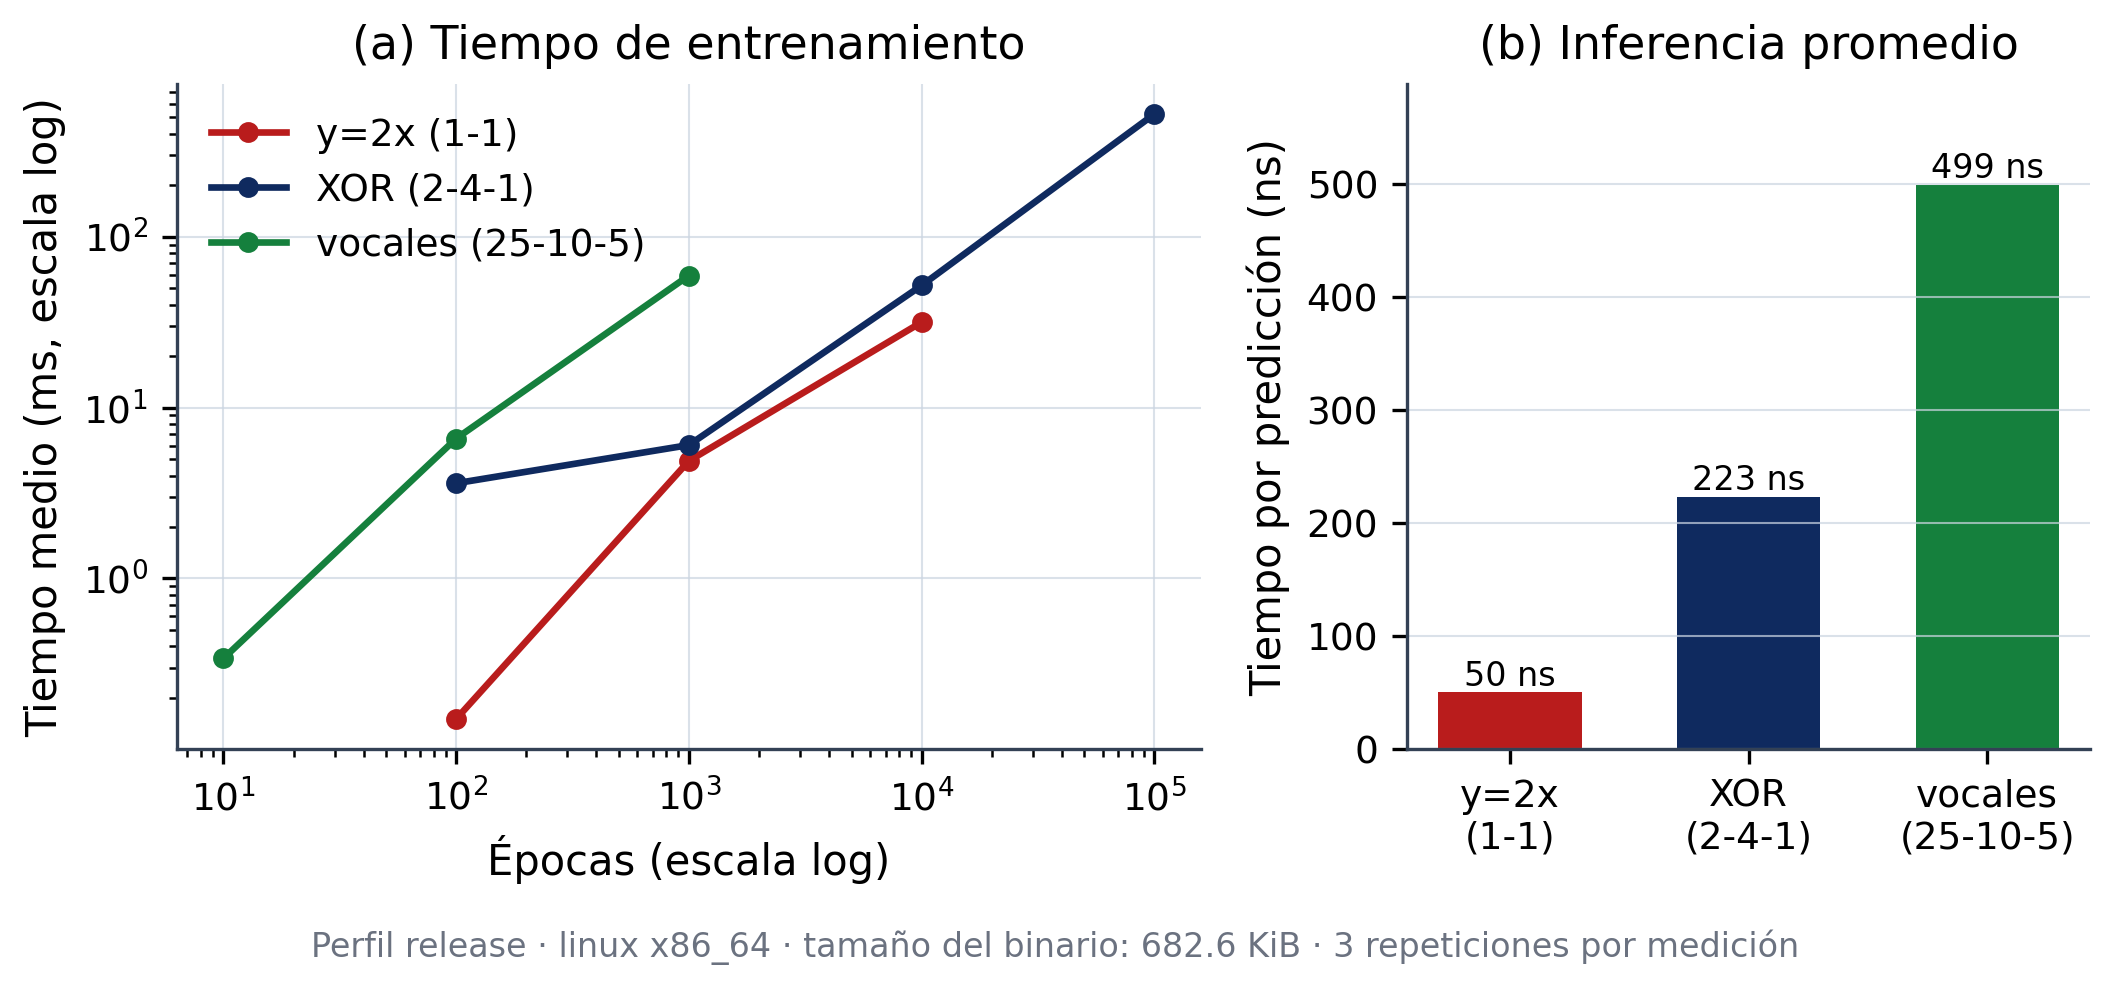
\includegraphics[width=\textwidth]{figuras/fig10_benchmarks_rust.png}
\fuente{(a) Tiempo medio de entrenamiento según el número de épocas, en escala logarítmica. (b) Tiempo medio por predicción. Fuente: \path{resultados/benchmarks.csv}.}
\end{figure}

El costo por época se mantiene aproximadamente constante para cada arquitectura una vez superadas las primeras ejecuciones, en las que influyen efectos de calentamiento de la caché, lo que confirma la complejidad lineal $O(E\cdot N\cdot P)$ del entrenamiento. La inferencia crece con el número de parámetros: la red de vocales, con 315 parámetros, requiere más tiempo por predicción que la red XOR de 17 parámetros, y ambas operan en el orden de los cientos de nanosegundos. Incluso 100\,000 épocas de XOR se completan en menos de un segundo, lo que demuestra que no se requiere hardware especializado para estudiar estos fundamentos.
